\section{Introduction}
\label{sec:intro}


Traditionally, writing a program is a relatively static process: a programmer writes some code and, after a successful compilation, can observe and inspect its behavior. If the code does not actually implement the programmer's intentions, they can correct the program and repeat the process.

\begin{marginfigure}
	\setlength{\abovecaptionskip}{0.1pt plus 0.1pt minus 0.1pt}
	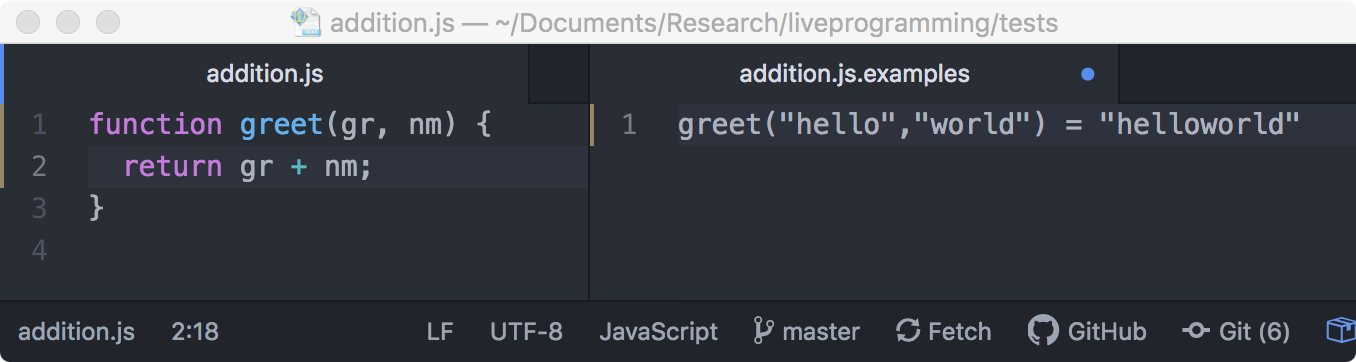
\includegraphics[width=0.55\textwidth]{figures/initial_greet}
	\caption{Code is written in the left hand panel,
	while examples are shown in the right hand panel.}
	\label{fig:init}
\end{marginfigure}
\begin{marginfigure}
	\setlength{\abovecaptionskip}{0.1pt plus 0.1pt minus 0.1pt}
	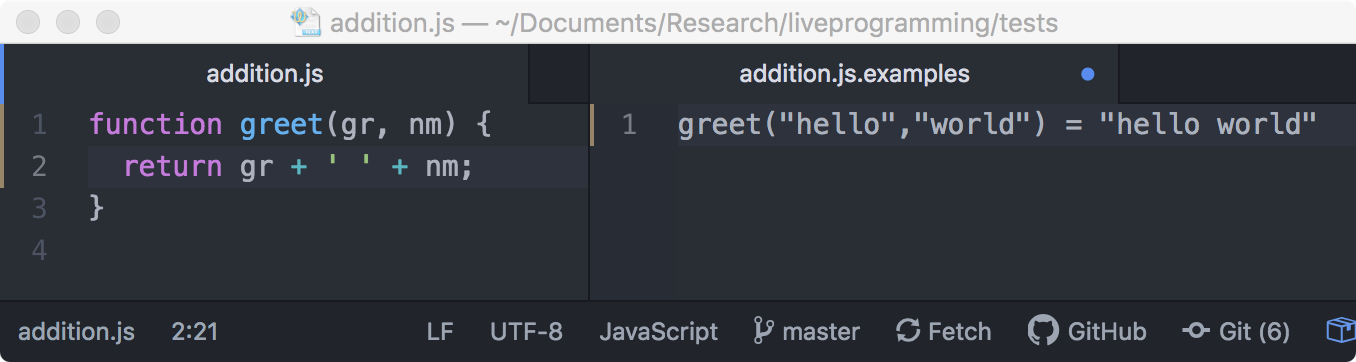
\includegraphics[width=0.55\textwidth]{figures/manual_change}
	\caption{When the code is modified, the examples update in real time.
	Here, the user has added a space to the output, by editing the code.}
	\label{fig:man_change}
\end{marginfigure}
\begin{marginfigure}
	\setlength{\abovecaptionskip}{0.1pt plus 0.1pt minus 0.1pt}
	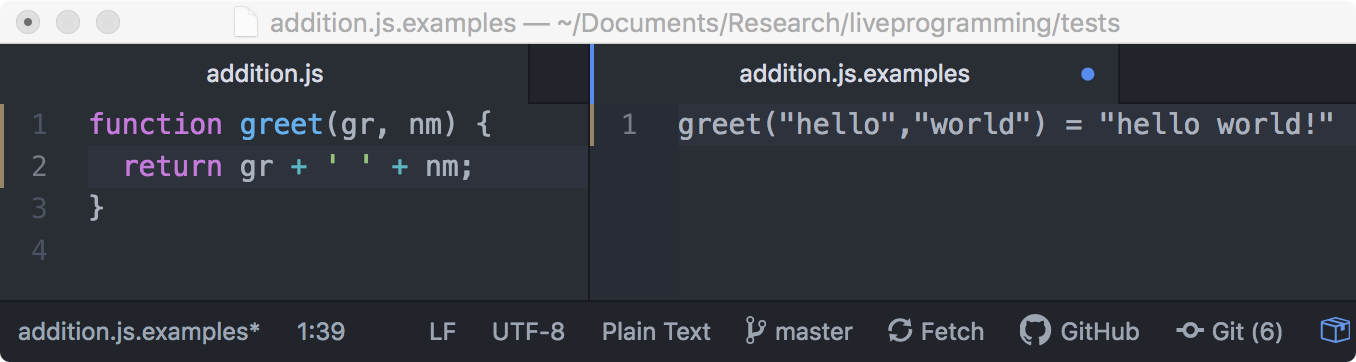
\includegraphics[width=0.55\textwidth]{figures/pbe_before}
	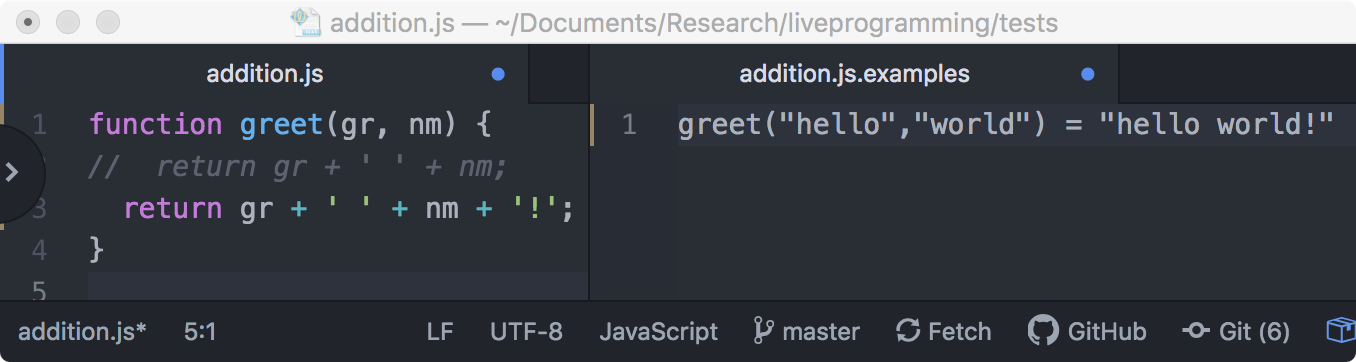
\includegraphics[width=0.55\textwidth]{figures/pbe_after}
	\caption{The user can also modify the output examples, to repair the code.  Here, the
	user has added a exclamation point to the end of the example's output, resulting in new code that appends an exclamation point.  The old code is preserved in a comment.}
	\label{fig:pbe}
\end{marginfigure}

Of course, this cycle often extends over a long period of time.
Not all bugs are discovered immediately,
and old code often has to be updated to suit new purposes.
Unfortunately, documentation is often incorrect or out of date,
leaving the best resource for developers as the code itself~\cite{latoza2006maintaining}.
In fact, it is estimated that half of a programmers time
is spent just \textit{comprehending} previously written code~\cite{corbi1989program}.

The live programming paradigm advocates a more dynamic programming cycle that allows the programmer to inspect and understand the code as it is written. As code is written, the user interface gives real-time feedback.  While existing live programming environments~\cite{victor2012, chugh2016programmatic, brown2009interacting} focus on programs with graphical or auditory output, we focus on general-purpose live programming.

We seek to give programmers immediate feedback as they write code,
an understanding of code that was written in the past, 
and a way to avoid manually writing code altogether.
We accomplish these goals through input/output examples.
We use \textit{live debugging} to show realtime feedback via changing outputs to fixed inputs as a function is modified.
We also leverage recent advances in \textit{programming by example} (PBE) to offer automated repairs based on input/output examples.

Both live debugging and PBE are also beneficial when \textit{later} modifying the code.
As opposed to traditional documentation, the live debugging examples update automatically, and thus will never fall out of date.
PBE simplifies modifying legacy code, by allowing programmers to simply demonstrate new behavior.
Of course, the programmer must be careful that desired existing behavior is preserved,
but this can be done by comparing the old and new code,
rather than having to write new code manually.

% Bill: I'm cutting this because, on rereading, I don't think it actually makes sense.  The examples for live debugging are exactly what is used in synthesis, so you're not going to discover an error by looking at them.  The synthesized program will never change them.
% PBE makes use of examples as an easily readable and understandable specification. However, even if the synthesized program satisfies all the provided examples, it still might not correspond to the user's intentions. Examples are, by nature, an incomplete specification. However, since live debugging allows a programmer to immediately and continuously see the effects of changes, the user can provide new examples that better illustrate their intentions when synthesis fails. The synthesized program is then refined with each new example. We call this approach {\emph{cooperative programming}}.

As an implementation, we developed a Javascript live coding plugin for the Atom text editor~\cite{Atom}.

% We introduce \textit{live debugging} as a technique to show realtime feedback as programmers write code.
% Programmers can specify an arbitrary number of function inputs,
% which are executed in realtime as they write and modify functions.
% By observing changes in the input-output pairs,
% the user receives immediate feedback about whether the code is correct without actually analyzing it in detail.
% Any example that behaves unexpectedly acts as a real-time indication of an error in the code. 

% Our framework also allows for \textit{programming by example}~\cite{cypher93,lieberman01,synasc12}.
% PBE  is a synthesis technique that automatically generates programs that coincide with given examples. An example is specified as a tuple of input and output values. Given a set $S= \{(i_1, o_1),\ldots, (i_n, o_n)\}$ of input/output examples, the goal is to automatically derive a program $P$ such that for every $j$, $P(i_j) = o_i$. The success and impact of this line of work can be seen from the fact that some of this technology ships as part of the popular Flash Fill feature in Excel 2013~\cite{flashFillPOPL}.

% Live debugging and programming by example naturally complement each other.
% Programming by example makes use of examples as an easily readable and understandable specification. However, even if the synthesized program satisfies all the provided examples, it still might not correspond to the user's intentions. Examples are, by nature, an incomplete specification. However, since live debugging allows a programmer to immediately and continuously see the effects of changes, the user can provide new examples that better illustrate their intentions when synthesis fails. The synthesized program can then be refined with each new example. We call this approach {\emph{cooperative programming}}.

% By combining live debugging and programming by example,
% our methodology offers programmers a useful work environment.
% Live debugging offers rapid feedback as code is written and modified. 
% When the user encounters unexpected output, they have two options.
% The user can go back to the code, detect
% the source of the error, and correct it manually.
% However, they can also adjust that output value directly,
% and rely on programming by example to ensure the program gives the expected output.

% A live programming environment is obtained through a standard
% Haskell REPL (Read Evaluate Print Loop) paradigm. 

% \noindent\fbox{%
%     \parbox{\textwidth}{%
% A small demo of our envisioned approach is available in the following video \\
% $\qquad$\url{https://www.youtube.com/watch?v=w5aI3N4dq2w}.    }%
% }

% \begin{figure}[h!]
% \centering
% \includegraphics[scale=0.5]{tool}
% \caption{A user interface for a live programming environment.}
% \label{fig:tool}
% \end{figure}


% The next question is how to correct the error? The user can go back to the code, detect
% the source of the error and correct it manually. We, additionally, want to offer an 
% automated repair by integrating recent advances in the PBE paradigm into this framework.
% If the user notices that the current program for an input value $i$ returns an incorrect value $o$, then she can adjust that value to specify that her intended program should return $o'$ instead.
% This feedback could allow a tool to automatically synthesize a program which coincides with all given examples (included the modified ones) and which follows the structure of the original code as closely as possible.
